% Figure from MATH 556 notes, section 24. Compile with the notes preamble.
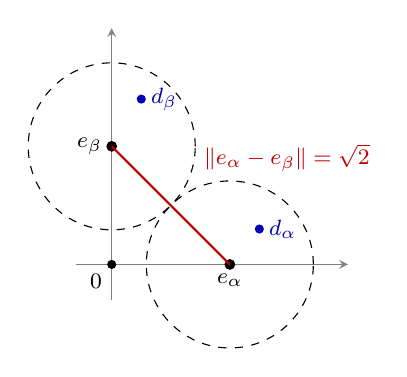
\begin{tikzpicture}[scale=1.5, >=stealth]
    \draw[->, thin, gray] (-0.3,0) -- (2.0,0);
    \draw[->, thin, gray] (0,-0.3) -- (0,2.0);
    \draw[dashed] (1,0) circle (0.707);
    \draw[dashed] (0,1) circle (0.707);
    \fill (1,0) circle (1.3pt) node[below, font=\footnotesize] {$e_\alpha$};
    \fill (0,1) circle (1.3pt) node[left, font=\footnotesize] {$e_\beta$};
    \draw[red!75!black, thick] (1,0) -- (0,1);
    \node[anchor=south west, font=\footnotesize, red!75!black] at (0.7,0.7) {$\|e_\alpha - e_\beta\| = \sqrt{2}$};
    \fill[blue!70!black] (1.25,0.3) circle (1.1pt) node[right, font=\footnotesize] {$d_\alpha$};
    \fill[blue!70!black] (0.25,1.4) circle (1.1pt) node[right, font=\footnotesize] {$d_\beta$};
    \fill (0,0) circle (1.1pt) node[below left, font=\footnotesize] {$0$};
\end{tikzpicture}
